\subsubsection{Wheel base}
\begin{itemize}
\item Since the robot is only supposed to do one task well, the structure of all the elements had to be optimized for the completion of that one task: collecting debris and placing it in the bins.

\item The decision not to pursue completion of other tasks means that we can use some additional motors to boost speed driving speed as well as improve climbing the ramp, bringing their number up from the usual four to six.

\item It was decided use six standard wheels. It allow high traction so we can climb to the ramp very well. The central wheel should be located near the COG of the robot. It allow fast and accurate turning. 

\item The U-contour was chosen as the shape of the wheelbase due to its proven durability and the ease with which other elements may be attached to it.

\item The use of a chain to connect the motors and wheels allows for more mobility in changing the position of the wheel, especially since the length of the chain can be changed freely.

\item The important moment is that chain should touch a half of circle of the gear. Otherwise it can slip during working. So it was decided to locate gears as in the picture
\begin{figure}[H]
	\begin{minipage}[h]{1\linewidth}
		\center{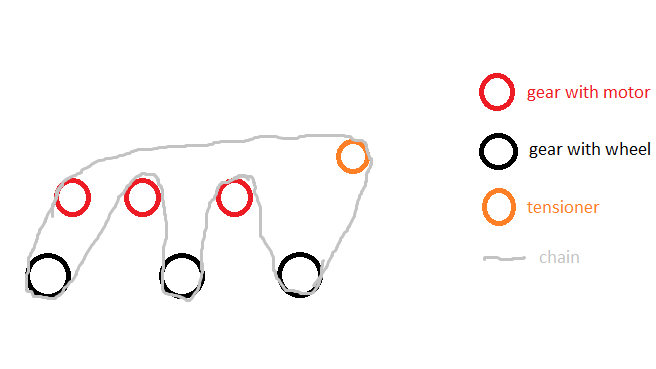
\includegraphics[scale=0.8]{days_L/Wheel_base/images/01}}
		\caption{Location of gears for chain}
	\end{minipage}
\end{figure} 



\item The first step in creating the wheelbase was making a model in Creo Parametric. Though in subsequent assembly the original design was deviated from, creating this model allowed us to establish a conceptual foundation that we were not to steer away from - usually doing so wastes time and effort.

\item To assemble the wheelbase, we needed to shorten a bar and create a chain of the exact length that was needed. In addition, the chain would slack on it's highest segment, and required careful adjustment to ensure that it would not slip while operating.

\item During tests and first competition we identified several problems:
	\begin{enumerate}
		\item Robot can't climb to ramp due to an overextension that prevented the robot from achieving the needed angle. And even if the robot was manually placed on the ramp on the needed position, it couldn't climb on top of the first churro due to low clearance. In order to fix this problem the front wheels were moved slightly forward, so that the distance between the wheel axis and the end of the beam would not exceed a certain value that is easily calculated through the angle of the ramp. After this was done, the robot could easily ride up the mountain. In order to fix the churro problem, we attached treads to the back wheels of the robot. This worked, but doing the same to all six wheels of the robot improved performance even further, and we could easily climb over the first churro in tests. However, when attempting to climb over the second churro, we found that our wheels were placed too close together:  the middle wheels pushed into the first churro and prevented the back ones from reaching the second one, and the robot would be unable to advance any further.
		
		\item Another problem we faced in first competition was the fact that our chain was not protected, and our robot could be disabled very easily just by driving into it and pulling the chain off. We added a metal sheet in front of the most exposed section of chain to protect it.
		
	\end{enumerate}
	\begin{figure}[H]
		\begin{minipage}[h]{\linewidth}
			\center{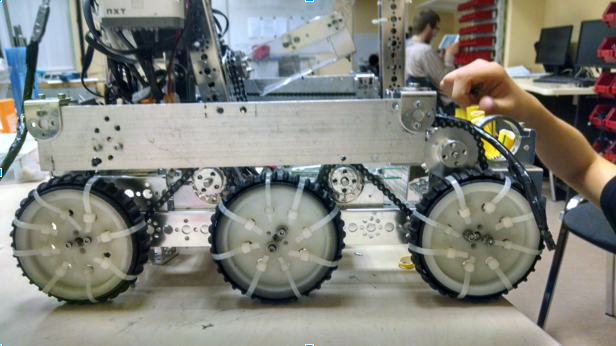
\includegraphics[scale=0.7]{days_L/Wheel_base/images/02}}
			\caption{Wheels with caterpillars and protection for chains}
		\end{minipage}
	\end{figure}
\end{itemize}
\fillpage
 
